% Standalone source. From the repository root:
% mkdir -p build/obstacle-map-notes
% latexmk -pdf -interaction=nonstopmode -halt-on-error \
%   -outdir=build/obstacle-map-notes Documentation/obstacle_map_method.tex
\documentclass[11pt,a4paper]{article}
\usepackage[T1]{fontenc}
\usepackage[utf8]{inputenc}
\usepackage{lmodern}
\usepackage[margin=25mm]{geometry}
\usepackage{amsmath,amssymb,mathtools}
\usepackage{booktabs,longtable,array}
\usepackage{enumitem}
\usepackage{microtype}
\DisableLigatures{encoding = T1, family = lmtt}
\usepackage{xcolor}
\usepackage{tikz}
\usetikzlibrary{arrows.meta}
\usepackage{algorithm}
\usepackage{algpseudocode}
\usepackage[section]{placeins}
\usepackage[colorlinks=true,linkcolor=blue!45!black,urlcolor=blue!45!black,
  citecolor=blue!45!black]{hyperref}
\hypersetup{pdftitle={Obstacle maps: geometry, finite elements, and the solver},
  pdfsubject={Technical explanation of the CutFEM obstacle-map implementation}}
\setlength{\parskip}{4pt}
\setlength{\emergencystretch}{1em}
\setlength{\parindent}{0pt}
\setlist{itemsep=2pt,topsep=4pt}
\setcounter{tocdepth}{1}
\newcommand{\R}{\mathbb R}
\newcommand{\dd}{\,\mathrm d}
\newcommand{\ip}[2]{\langle #1,#2\rangle_g}
\newcommand{\norm}[1]{\lVert #1\rVert}
\newcommand{\code}[1]{\texttt{\detokenize{#1}}}
\newcommand{\conv}{\operatorname{conv}}
\newcommand{\diag}{\operatorname{diag}}
\newcommand{\Hess}{\operatorname{Hess}}
\newcommand{\divg}{\operatorname{div}_g}
\newcommand{\tr}{\operatorname{tr}}
\newcommand{\free}{\mathcal I}
\newcommand{\collar}{\mathcal C_h}
\newcommand{\bulk}{\mathcal B_h}

\title{Obstacle maps:\\geometry, finite elements, and the solver}
\author{Technical notes for discussion with a PI}
\date{Implementation inspected: 18 October 2026}

\begin{document}
\maketitle

\begin{abstract}
An obstacle map minimizes Dirichlet energy while its values remain in an
admissible target manifold with boundary. The implementation represents the
map by coordinates \(q=(s,r)\), with the obstacle expressed as \(r\geq0\).
It interpolates these coordinates with conforming piecewise affine finite
elements and evaluates the physical map as \(u_h=F(q_h)\). The resulting
nonlinear constrained energy is reduced by successive normal, tangential,
and bulk updates. Each update solves a convex quadratic model and undergoes
a feasibility check and an energy line search. These notes derive the
equations, explain the algorithm, and distinguish continuum geometry,
finite-dimensional mathematics, and C++ storage. The implementation is a
fitted finite element method in the CutFEM repository.
\end{abstract}

\tableofcontents
\clearpage

\section{The central idea and the three levels of description}
\label{sec:idea}

The description follows the inspected implementation \cite{implementation}.
The unknown is a \emph{map}: each source point \(x\in\Omega\) is assigned a
target point \(u(x)\). The obstacle is a restriction on target values.
The source is still meshed throughout its contact and noncontact regions.
The contact set is the part of the source mapped onto the target boundary;
its boundary inside the source is the free boundary to be discovered.

The method uses target coordinates to turn geometric feasibility into a
scalar lower bound. Near the target boundary, \(s\) locates the nearest
boundary point and \(r\) is the inward distance into the admissible target.
Changing \(r\) changes contact; changing \(s\) moves the map along the target
boundary or a parallel hypersurface. Both changes affect the same energy.
Away from contact, the stationary map satisfies the harmonic-map equation.

Three levels must be kept distinct:
\begin{enumerate}
  \item \textbf{Continuum mathematics:} manifolds, metrics, Sobolev maps,
  energy, first variations, and a contact reaction.
  \item \textbf{Discrete mathematics:} a mesh, a finite element space,
  nodal coefficients, a finite element energy, its derivative, and
  constrained quadratic minimization problems.
  \item \textbf{Data structures:} mesh classes, vectors, sparse containers,
  callbacks, and Boolean masks representing the preceding objects.
\end{enumerate}
For example, a Riemannian metric is a field of inner products. Its coordinate
matrix is a mathematical representation of that field; a flat array holding
the matrix entries is a data structure. Likewise, the map \(u\), the
coefficient vector \(Q\), and a C++ \code{std::map} are three different things.

Sections~\ref{sec:geometry}--\ref{sec:continuum} describe the mathematical
problem. Sections~\ref{sec:discrete}--\ref{sec:stopping} describe the numerical
method. Section~\ref{sec:storage} connects those objects to the implementation.

\clearpage
\section{Geometry, coordinates, and the admissible class}
\label{sec:geometry}

\subsection{Data supplied by the user}
\label{sec:input-data}
The following table lists the inputs to a problem specification. Here
\(\Omega\) is the source, \(\overline M\) is the admissible target,
\(q=(s^1,\ldots,s^{m-1},r)\) denotes target coordinates, and \(u=F(q)\).
The label \emph{Required} means that the specification must provide the
data, possibly through an existing mesh or geometry helper. Mathematical
data and the callbacks or containers representing them are listed separately.

\begingroup
\small
\setlength{\tabcolsep}{4pt}
\begin{longtable}{@{}>{\raggedright\arraybackslash}p{.19\textwidth}
 >{\raggedright\arraybackslash}p{.42\textwidth}
 >{\raggedright\arraybackslash}p{.35\textwidth}@{}}
\caption{Inputs to the obstacle-map solver and example driver.}
\label{tab:user-inputs}\\
\toprule
Input & Mathematical data and requirement & Interface and default \\
\midrule
\endfirsthead
\multicolumn{3}{@{}l}{\textit{Table \thetable\ continued: user-supplied inputs}}\\
\toprule
Input & Mathematical data and requirement & Interface and default \\
\midrule
\endhead
\midrule
\multicolumn{3}{r@{}}{\textit{Continued on the next page}}\\
\endfoot
\bottomrule
\endlastfoot
Source dimension and mesh, \(D,\mathcal T_h\) &
\textbf{Required.} A fitted triangular (\(D=2\)) or tetrahedral (\(D=3\))
mesh of \(\Omega_h\), including vertices, connectivity, and boundary
elements. Cells must have positive, consistent measures. All boundary
vertices receive Dirichlet data. &
\code{Mesh2} or \code{Mesh3}, passed to \code{ObstacleMapProblem<D>}
or \code{.on(mesh)}. A mesh generator may supply these data from dimensions
and a resolution choice. \\
\addlinespace
Source metric, \(g\) &
Supply \(g^{-1}(x)\) and the consistent volume density
\(\sqrt{\det g(x)}\) for a non-Euclidean source. &
Optional \code{Source} callback returning \code{SourceMetric<D>}.
Default: Euclidean metric and density \(1\). The fluent example driver uses
this default; a custom source uses the problem constructor directly. \\
\addlinespace
Target dimension and coordinate convention, \(m,q\) &
\textbf{Required choice.} \(m\geq1\); the last coordinate is \(r\).
Boundary and initial data must use the same coordinate representation,
including a compatible lift if the parameterization is a covering. &
\code{TargetChart::dimension} (member default \(2\)).
Every coordinate callback returns \(m\) components. \\
\addlinespace
Target parameterization, \(F\) &
\textbf{Required.} A regular representation of the entire computed image,
with \(r=0\) representing the obstacle boundary and \(r\geq0\) the feasible
side. Near contact it must follow the Fermi convention. &
\code{TargetChart::embed(q)}, or the value component of an
\code{EmbeddingJet}. For an intrinsic target, the returned vector may be
a display representation; its Euclidean metric need not be the target metric. \\
\addlinespace
Target metric, \(G\), and derivatives, \(\partial_cG\) &
\textbf{Required, directly or through the embedding helper.} Supply the
full positive definite \(m\times m\) metric and its first derivatives in
every target coordinate, consistently with the chosen geometry. &
\code{TargetChart::metric(q,G,dG)}. Alternatively,
\code{embeddedTargetChart} computes them from a Euclidean isometric
embedding and its derivatives; see the paragraph below. \\
\addlinespace
Collar width, \(\delta\) &
\textbf{Required geometric choice.} A positive width on which \(r\) is
inward geodesic distance and the Fermi representation is valid.
The solver does not estimate reach or locate a cut locus. &
\code{TargetChart::tube_radius}. Bare member default: \(0.05\).
Example-driver default: \(0.03\), adjustable with \code{--tube}.
Any default must be valid for the supplied geometry. \\
\addlinespace
Valid coordinate domain and element certificate &
\textbf{Required.} A criterion certifying that each entire coordinate
simplex hull stays in the regular representation and maps into
\(\overline M\). Vertex or quadrature samples alone are insufficient
without an argument covering the whole hull. &
The target's \code{admissible_simplex} callback.
The valid domain is encoded by this callback; there is no separate
domain object or automatic construction of the certificate. \\
\addlinespace
Dirichlet trace, \(q_D\) &
\textbf{Required.} Prescribed target \emph{coordinates} on the source
boundary, with nonnegative \(r_D\) and a compatible global lift.
The induced discrete trace must satisfy the element certificate. &
The \code{boundary} callback in \code{solve}, or
\code{.withDirichlet(...)}. Evaluated only at boundary vertices.
Physical values \(u_D\) must first be expressed in the chosen coordinates. \\
\addlinespace
Initial coordinates, \(q^{(0)}\) &
\textbf{Required.} A starting coordinate field. After interpolation and
overwriting boundary coefficients with \(q_D\), the full field must have
\(r_I\geq0\) and satisfy the element certificate. &
The \code{initial} callback in \code{solve}, or
\code{.startingFrom(...)}. The solver does not construct a feasible
initial extension of the trace. \\
\addlinespace
Iteration controls &
Optional choices of outer and inner tolerances, step regularization
\(\sigma\), line-search parameters, iteration limits, number of bulk
sweeps, and output contact tolerance. &
\code{ObstacleMapOptions}, or \code{.usingSolver(...)}.
Defaults exist for every control; their values and meanings are given
in Section~\ref{sec:stopping}. \\
\addlinespace
Reference map, \(q_{\rm ref}\) &
Optional coordinate-valued reference for error measurement.
It is not used to compute the solution. &
\code{.compareWith(...)} in the example driver.
Default: no reference comparison. \\
\addlinespace
Output destination &
Optional filename prefix for the driver's VTK and CSV files. &
\code{.writeTo(prefix)} or \code{--output}.
Default: \code{obstacle_map}. The core problem solver itself returns
an \code{ObstacleMapResult} without writing files. \\
\addlinespace
Iteration monitor &
Optional callback receiving current diagnostics during the solve. &
The final \code{monitor} argument of \code{solve}.
Default: none in the core solver; the example driver supplies console
reporting. \\
\end{longtable}
\endgroup

\textbf{Two ways to supply target geometry.}
With a direct \code{TargetChart}, provide \(F\), \(G\), and every
\(\partial_cG\) through the callbacks above. With
\code{embeddedTargetChart}, instead provide the target dimension \(m\),
Euclidean embedding dimension \(p\geq m\), a callback returning
\((F,DF,D^2F)\), the collar width, and the element certificate.
The helper constructs \code{embed} and \code{metric}; separate metric
derivatives are then unnecessary. This alternative requires an isometric
Euclidean embedding. In either route, constructing the valid
parameterization and choosing a valid collar remain part of problem setup.

Neither a contact set nor a free boundary is prescribed. The algorithm
computes the contact labels and collar-node mask from the coordinate field.
In particular, \(\delta\) is supplied but the element patch selected by
\(r_h<\delta\) is recomputed during iteration
(Section~\ref{sec:algorithm}). The basis functions, degree-two quadrature,
assembled derivative, step matrices, and reactions are also constructed
by the implementation.

\subsection{Source, target, and dimensions}
Let \((\Omega,g)\) be the source, of dimension \(D\), and let
\((\widehat M,h)\) be an ambient Riemannian target of dimension \(m\).
Let \(M\subset\widehat M\) be the admissible open region and
\(\Sigma=\partial M\) its smooth boundary. The map takes values in
\(\overline M\). If \(\widehat M\) is realized isometrically in Euclidean
space, denote that ambient Euclidean dimension by \(p\).

\begin{center}
\begin{tabular}{lll}
\toprule
Symbol & Meaning & Spherical-cap example \\
\midrule
\(D\) & Source dimension & \(3\): a ball \\
\(m\) & Target coordinate dimension & \(2\): a surface \\
\(p\) & Euclidean embedding dimension, when used & \(3\): \(S^2\subset\R^3\) \\
\bottomrule
\end{tabular}
\end{center}
Thus a three-dimensional source can map into a two-dimensional target.
The solver supports \(D=2,3\), with \(m\geq1\) chosen at run time. It
assembles using the intrinsic target metric; an embedding is not required
to define that energy.

\subsection{The Fermi representation}
Let \(\rho\) be signed distance to \(\Sigma\), positive inside \(M\), in a
regular tubular neighborhood. Let \(\nu=\nabla^h\rho\) point into \(M\),
and let \(\gamma(s)\) parameterize a portion of \(\Sigma\). Define
\begin{equation}
 F(s,r)=\exp_{\gamma(s)}(r\nu_{\gamma(s)}),\qquad
 q=(s^1,\ldots,s^{m-1},r),\qquad u=F\circ q.
 \label{eq:fermi}
\end{equation}
Here \(F\) is the coordinate-to-target map, sometimes called the chart
parameterization; strictly, the corresponding coordinate chart is its local
inverse. In the collar, \(r=\rho\circ u\), and
\(v=\gamma\circ s=\Pi_\Sigma\circ u\) is a manifold-valued boundary map.
The vector \(s\) contains coordinates of \(v\); it is not itself a tangent
vector. The manuscript writes the same decomposition as \(u=E(v,r)\)
\cite{regularity}.

The pullback metric has coefficients
\begin{equation}
 G_{ab}(q)=h_{F(q)}(\partial_a F,\partial_b F),\qquad
 G(s,r)=\begin{pmatrix}A(s,r)&0\\0&1\end{pmatrix}
 \quad\text{in the Fermi collar}.
 \label{eq:metric}
\end{equation}
The matrix \(A\) has size \((m-1)\times(m-1)\). Only when \(m=2\) can it
be described by a single scalar coefficient. The identities
\(G_{rr}=1\) and \(G_{\alpha r}=0\) express unit normal speed and
orthogonality. They do not imply that tangential and normal variations
decouple: \(A\) generally depends on \(r\).

The implementation requires one regular coordinate representation over the
\emph{entire computed image}. Beyond the declared collar, \(r\) may be a
nonnegative defining coordinate instead of distance; \(G\) may then have
normal--tangential cross terms. A Fermi map cannot simply be extended through
a focal point or cut locus. The geometry provider must supply a valid extension
and certify the coordinate images of whole source elements.

A periodic parameterization, such as unwrapped longitude, is also usable if
the map admits a single continuous coordinate lift. This permits a covering
parameterization without requiring global injectivity. It does not provide
an atlas or represent every possible topological class. For example, angular
data with incompatible winding need not admit a real-valued global angle.

\subsection{Energy, contact, and boundary data}
Fix an admissible source-boundary trace \(q_D\). Within the chosen
representation the admissible class is
\begin{equation}
 \mathcal K=\{q\in H^1(\Omega;\R^m):q|_{\partial\Omega}=q_D,\;
 r\geq0\text{ a.e.},\;q\text{ takes values in the valid coordinate domain}\}.
 \label{eq:admissible}
\end{equation}
Finite energy and appropriate regularity of the representation are understood.
The energy and minimization problem are
\begin{equation}
 E(q)=\frac12\int_\Omega G_{ab}(q)g^{ij}\partial_iq^a\partial_jq^b\dd V_g,
 \qquad \min_{q\in\mathcal K}E(q),\qquad
 \dd V_g=\sqrt{\det g}\dd x.
 \label{eq:energy}
\end{equation}
Repeated indices are summed: \(i,j=1,\ldots,D\),
\(a,b,c=1,\ldots,m\), and Greek indices run through \(1,\ldots,m-1\).
Write \(\ip{\nabla f}{\nabla w}=g^{ij}\partial_i f\partial_j w\).
The energy measures spatial variation of the map using both metrics.
Although \(r\geq0\) is a linear coordinate inequality, \(E\) is generally
nonconvex because \(G\) depends on \(q\).

For a continuous map define
\begin{equation}
 C=\{x\in\Omega:r(x)=0\},\qquad
 O=\{x\in\Omega:r(x)>0\},\qquad
 \Gamma=\partial_\Omega O.
\end{equation}
The target obstacle boundary \(\Sigma\), source contact set \(C\), and
source free boundary \(\Gamma\) are distinct geometric sets. At lower
regularity these notions require appropriate representatives; the numerical
coordinate field is continuous.

\section{First variation, curvature, and complementarity}
\label{sec:continuum}

\subsection{The full coordinate variation}
For a variation \(w\) with zero source-boundary trace, differentiate both
the metric and the coordinate derivatives in~\eqref{eq:energy}. Symmetry of
\(G\) combines the two derivative terms, giving
\begin{equation}
 DE(q)[w]=\int_\Omega
 G_{cb}(q)\ip{\nabla w^c}{\nabla q^b}
 +\frac12\partial_cG_{ab}(q)w^c\ip{\nabla q^a}{\nabla q^b}\dd V_g.
 \label{eq:first-variation}
\end{equation}
Both terms are essential. Freezing \(G\) when computing the derivative
would discard the second term and solve a different problem. The code
includes derivatives with respect to every target coordinate and derivatives
of off-diagonal metric entries.

Where all variations are admissible, integration by parts gives
\begin{equation}
 \mathcal R_c(q)=
 -\divg\bigl(G_{cb}(q)\nabla_g q^b\bigr)
 +\frac12\partial_cG_{ab}(q)\ip{\nabla q^a}{\nabla q^b}=0.
 \label{eq:coordinate-residual}
\end{equation}
Equivalently, after multiplying by \(G^{-1}\),
\begin{equation}
 \Delta_g q^a+\Gamma^a_{bc}(q)\ip{\nabla q^b}{\nabla q^c}=0,
 \qquad
 \Gamma^a_{bc}=\tfrac12G^{ad}
 (\partial_bG_{dc}+\partial_cG_{db}-\partial_dG_{bc}).
 \label{eq:harmonic}
\end{equation}
These are harmonic-map equations. Componentwise Laplace equations result
for a Euclidean target in Cartesian coordinates; general target coordinates
retain the connection terms.

\subsection{The collar equations and the sign of the reaction}
In the collar,~\eqref{eq:energy} becomes
\begin{equation}
 E(s,r)=\frac12\int_\Omega
 \bigl(|\nabla r|_g^2+A_{\alpha\beta}(s,r)
 \ip{\nabla s^\alpha}{\nabla s^\beta}\bigr)\dd V_g,
 \label{eq:split-energy}
\end{equation}
when the image lies there; otherwise use this expression locally.
The normal and tangential variations are
\begin{align}
 \mathcal G_r[\eta]&=\int_\Omega
 \ip{\nabla r}{\nabla\eta}
 +\tfrac12\partial_rA_{\alpha\beta}
 \ip{\nabla s^\alpha}{\nabla s^\beta}\eta\dd V_g,
 \label{eq:normal-weak}\\
 \mathcal G_{s^\gamma}[\xi]&=\int_\Omega
 A_{\gamma\beta}\ip{\nabla s^\beta}{\nabla\xi}
 +\tfrac12\partial_{s^\gamma}A_{\alpha\beta}
 \ip{\nabla s^\alpha}{\nabla s^\beta}\xi\dd V_g.
 \label{eq:tangent-weak}
\end{align}
Tangential variations have both signs, so \(\mathcal G_s=0\). At contact,
normal variations may increase \(r\), but cannot decrease it below zero.
Thus \(\mathcal G_r[z-r]\geq0\) for feasible normal competitors \(z\)
with the same trace and a valid coordinate variation.

When the reaction has a density, this gives the Karush--Kuhn--Tucker
(KKT) conditions
\begin{equation}
 \boxed{\quad
 \lambda=-\Delta_g r+\tfrac12\partial_rA_{\alpha\beta}
 \ip{\nabla s^\alpha}{\nabla s^\beta}\geq0,
 \qquad r\geq0,\qquad r\lambda=0.\quad}
 \label{eq:kkt}
\end{equation}
The sign follows directly from a positive normal test at \(r=0\): moving
away from the obstacle must not lower the energy to first order. On \(O\),
both signs are available and \(\lambda=0\). In a weak formulation \(\lambda\)
may instead be a nonnegative measure supported on contact; a pointwise
multiplier formula then requires additional regularity \cite{regularity}.

To connect the notation to the manuscript, let
\(b_r(X,Y)=-\Hess^h\rho(X,Y)\) on the parallel target hypersurface.
In Fermi coordinates,
\begin{equation}
 (\Hess^h\rho)_{\alpha\beta}=\tfrac12\partial_r A_{\alpha\beta},
 \qquad
 H_r(dv,dv)=-\tfrac12\partial_r A_{\alpha\beta}
 \ip{\nabla s^\alpha}{\nabla s^\beta}.
\end{equation}
Hence \(\lambda=-(\Delta_g r+H_r(dv,dv))\), with densities interpreted
relative to \(\dd V_g\). The tangential strong equation can likewise be
written \(\tau_r(v)+2S_r(dv\,\nabla_g r)=0\), with
\(S_r(X)=\nabla^h_X\nu\), as in the manuscript. The coordinate weak
form~\eqref{eq:tangent-weak} already includes this coupling.

The geometric mechanism is visible in~\eqref{eq:kkt}: the variation of
the tangential metric with normal distance acts as a forcing term in the
normal obstacle problem. A scalar obstacle equation for \(r\) alone does
not determine the map, because this term also depends on the unknown \(s\).
The related distance/projected-image decomposition in the Euclidean
obstacle setting is discussed by Figalli, Kim, and Shahgholian
\cite{fks}. That work provides continuum regularity background; it is
not a specification of the numerical algorithm described here.

\section{Finite elements and the energy in integral form}
\label{sec:discrete}

In this section we discretize the coordinate field in a finite element
space while retaining spatial integrals in the energy and weak forms.
This is the semidiscrete description used here: numerical integration is
left implicit. The unknowns are still finitely many nodal coefficients.

\subsection{Interpolate coordinates, then evaluate the map}
Let \(\mathcal T_h\) be a fitted simplicial mesh of a polyhedral source
\(\Omega_h\), with \(N\) vertices and continuous P1 basis functions
\(\phi_I\). The scalar trial and test spaces are
\begin{equation}
 V_h=\{w_h\in C^0(\overline{\Omega_h}):
           w_h|_T\in\mathbb P_1(T)\text{ for every }T\in\mathcal T_h\},
 \qquad V_{h,0}=V_h\cap H^1_0(\Omega_h).
 \label{eq:fe-spaces}
\end{equation}
The coordinate field belongs to \(V_h^m\), and the discrete map is
\begin{equation}
 q_h(x)=\sum_{I=0}^{N-1}q_I\phi_I(x),\qquad
 u_h(x)=F\bigl(q_h(x)\bigr),\qquad q_I=(s_I,r_I)\in\R^m.
 \label{eq:interpolation}
\end{equation}
It is \(q_h\), rather than the ambient components of \(u_h\), that is
piecewise affine. Each simplex has nonnegative barycentric basis functions
summing to one. Consequently,
\begin{equation}
 r_I\geq0\ \text{at all vertices}
 \quad\Longrightarrow\quad
 r_h(x)=\sum_I r_I\phi_I(x)\geq0\ \text{throughout every element}.
 \label{eq:positivity}
\end{equation}
The geometry provider must additionally certify
\begin{equation}
 \conv\{q_I:I\text{ is a vertex of }T\}
 \subset \mathcal U_{\mathrm{valid}},\qquad
 F(\mathcal U_{\mathrm{valid}})\subset\overline M
 \quad(T\in\mathcal T_h).
 \label{eq:certificate}
\end{equation}
Testing only finitely many points is insufficient unless those
tests certify the entire hull, for example by containment in a known convex
coordinate region. Higher order nodal bases generally lose the positivity
argument~\eqref{eq:positivity}.

\begin{figure}[htbp]
\centering
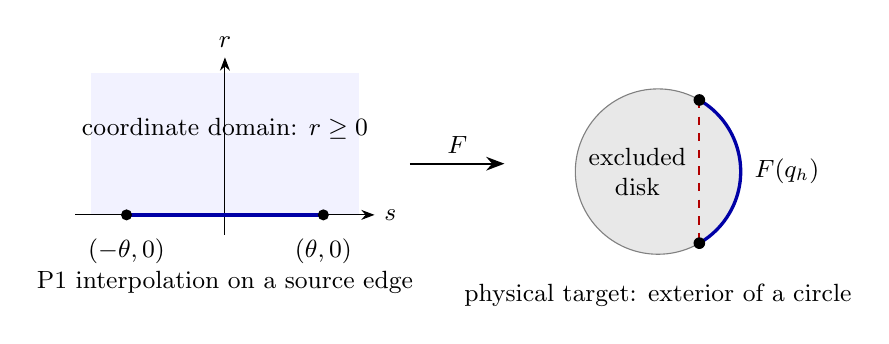
\begin{tikzpicture}[>=Stealth,font=\small]
  \begin{scope}[xshift=0cm]
    \fill[blue!5] (-1.7,0) rectangle (1.7,1.8);
    \draw[->] (-1.9,0)--(1.9,0) node[right] {\(s\)};
    \draw[->] (0,-.25)--(0,2) node[above] {\(r\)};
    \draw[very thick,blue!65!black] (-1.25,0)--(1.25,0);
    \fill (-1.25,0) circle (2pt) node[below=5pt] {\((-\theta,0)\)};
    \fill (1.25,0) circle (2pt) node[below=5pt] {\((\theta,0)\)};
    \node at (0,1.1) {coordinate domain: \(r\geq0\)};
    \node at (0,-.85) {P1 interpolation on a source edge};
  \end{scope}
  \draw[->,thick] (2.35,.65)--(3.55,.65) node[midway,above] {\(F\)};
  \begin{scope}[xshift=5.5cm,yshift=.55cm,scale=1.05]
    \fill[gray!18] (0,0) circle (1);
    \draw[gray] (0,0) circle (1);
    \draw[very thick,blue!65!black] (60:1) arc[start angle=60,end angle=-60,radius=1];
    \draw[thick,dashed,red!70!black] (60:1)--(-60:1);
    \fill (60:1) circle (2pt);
    \fill (-60:1) circle (2pt);
    \node[align=center] at (-.25,0) {excluded\\disk};
    \node[right] at (1.05,0) {\(F(q_h)\)};
    \node[align=center] at (0,-1.5) {physical target: exterior of a circle};
  \end{scope}
\end{tikzpicture}
\caption{For \(F(s,r)=((1+r)\cos s,(1+r)\sin s)\), interpolating
\((-\theta,0)\) and \((\theta,0)\) in coordinates traces the admissible
blue arc. Ambient linear interpolation traces the dashed chord through the
excluded disk. Its midpoint has radius \(\cos\theta<1\), whereas
\(F(0,0)=(1,0)\). This is a schematic edge illustration, not a computed result.}
\label{fig:interpolation}
\end{figure}

Boundary coefficients are prescribed at all mesh-boundary vertices. The
coordinate trace on boundary facets is therefore the P1 interpolant of the
given nodal trace, denoted by \(q_{D,h}\). On a fitted polyhedral ball, neither the source boundary
nor this interpolated trace is the exact curved continuum boundary data.

\subsection{Finite element energy and its derivative}
Use \(Q\in\R^{Nm}\) for the vector of all \(q_I\). The finite element
energy is the Dirichlet energy restricted to coordinate fields in \(V_h^m\):
\begin{equation}
 E_h(Q)=\frac12\int_{\Omega_h}
 G_{ab}(q_h)\ip{\nabla q_h^a}{\nabla q_h^b}\dd V_g.
 \label{eq:discrete-energy}
\end{equation}
The admissible fields have trace \(q_{D,h}\), nonnegative nodal normal
coordinates, and valid coordinate hulls as in~\eqref{eq:certificate}.
Minimizing~\eqref{eq:discrete-energy} over these fields is a
finite-dimensional constrained variational problem, even though its
objective is written as an integral.

Let \(w_h=\sum_I W_I\phi_I\in V_{h,0}^m\) be a coordinate variation.
Restricting the continuum first variation~\eqref{eq:first-variation}
to this test space gives
\begin{align}
 DE_h(Q)[W]
 &=\int_{\Omega_h}
 \Bigl[G_{cb}(q_h)\ip{\nabla w_h^c}{\nabla q_h^b}
 \nonumber\\[-2pt]
 &\hspace{20mm}
 +\tfrac12\partial_cG_{ab}(q_h)w_h^c
       \ip{\nabla q_h^a}{\nabla q_h^b}\Bigr]\dd V_g.
 \label{eq:discrete-first-variation}
\end{align}
The coefficient derivative \(f_{I,c}=\partial E_h/\partial q_I^c\)
is obtained by taking the test function \(\phi_I e_c\), where \(e_c\)
is the \(c\)-th coordinate vector in \(\R^m\):
\begin{align}
 f_{I,c}
 &=\int_{\Omega_h}
 \Bigl[G_{cb}(q_h)\ip{\nabla\phi_I}{\nabla q_h^b}
 \nonumber\\[-2pt]
 &\hspace{20mm}
 +\tfrac12\partial_cG_{ab}(q_h)\phi_I
       \ip{\nabla q_h^a}{\nabla q_h^b}\Bigr]\dd V_g.
 \label{eq:discrete-gradient}
\end{align}
Thus \(DE_h(Q)[W]=f^TW\). The vector \(f\) is the derivative of the
finite element energy with respect to its coefficients, rather than a
spatial gradient such as \(\nabla_g r_h\) or an \(L^2\) Riesz representative.
The same formula defines boundary rows, although only free-node test
functions are used for stationarity with the trace fixed.

\subsection{Frozen stiffness and lumped mass}
At the current map \(q_h\), define the bilinear form
\begin{equation}
 a_{q_h}(z_h,w_h)=\int_{\Omega_h}
 G_{ab}(q_h)\ip{\nabla z_h^a}{\nabla w_h^b}\dd V_g.
\end{equation}
The frozen-metric stiffness and the lumped source masses are
\begin{align}
 K_{Ia,Jb}(Q)&=\int_{\Omega_h}
 G_{ab}(q_h)\ip{\nabla\phi_I}{\nabla\phi_J}\dd V_g,
 \label{eq:stiffness}\\
 M_I&=\int_{\Omega_h}\phi_I\dd V_g,\qquad
 \mathsf M=\diag(M_0 I_m,\ldots,M_{N-1} I_m).
 \label{eq:mass}
\end{align}
These global integrals can equivalently be assembled as sums of element
integrals. The basis supports make the matrices sparse.

The mass remains \emph{lumped} in this integral formulation. Indeed, if
\(M^{\rm cons}_{IJ}=\int_{\Omega_h}\phi_I\phi_J\dd V_g\) is the consistent
scalar mass matrix, then the partition of unity gives
\(M_I=\sum_J M^{\rm cons}_{IJ}\). The solver uses these row sums on the
diagonal, repeated for each target coordinate. For a mesh with no unused
vertices and a positive source volume density, \(M_I>0\).

For a coefficient direction \(Z\) representing \(z_h\),
\begin{equation}
 Z^TK(Q)Z=a_{q_h}(z_h,z_h)
 =\int_{\Omega_h}G_{ab}(q_h)
       \ip{\nabla z_h^a}{\nabla z_h^b}\dd V_g\geq0.
\end{equation}
Thus \(K\) is positive semidefinite. It is generally \emph{not}
\(D^2E_h(Q)\): a full Hessian also differentiates \(G(q_h)\) and the
metric-derivative terms. The algorithm uses the true first derivative
with this simpler positive step metric.

\textit{Implementation note.}
The algorithm below is written using these integral quantities. In the
code, \(E_h,f,K,M\) are replaced consistently by their numerical-integration
counterparts, using a common quadrature rule. The assembled derivative
then differentiates that numerically integrated energy. Writing the
integrals here does not assert that the implementation evaluates them
exactly; the block structure and KKT conditions have the same form.

\subsection{Discrete stationarity}
Let \(\free\) be the set of non-Dirichlet vertices. In the interior of the
valid chart region, the discrete KKT conditions are
\begin{equation}
 f_{I,\alpha}=0,\qquad
 r_I\geq0,\qquad f_{I,r}\geq0,\qquad r_I f_{I,r}=0,
 \qquad I\in\free.
 \label{eq:discrete-kkt}
\end{equation}
They follow from the Lagrangian
\(L(Q,\mu)=E_h(Q)-\sum_{I\in\free}\mu_I r_I\), with
\(\mu_I=f_{I,r}\). Define the lumped multiplier
\(\lambda_I=f_{I,r}/M_I\), so
\(\sum_I f_{I,r}\eta_I=\sum_I M_I\lambda_I\eta_I\).
The code reports the corresponding numerically assembled multiplier as
reaction. Chart boundaries
are validity restrictions enforced by rejection, not additional KKT
constraints solved by the algorithm.

\section{The nonlinear solution algorithm}
\label{sec:algorithm}

\subsection{Collar and bulk select variables}
Let \(\delta>0\) be \code{tube_radius}. At the current iterate mark
\begin{align}
 \mathcal T_{\mathrm{near}}(Q)
 &=\{T\in\mathcal T_h:\min_{I\in T}r_I<\delta\},\\
 \collar(Q)&=\{I:I\text{ belongs to an element in }\mathcal T_{\mathrm{near}}(Q)\},
 \qquad \bulk(Q)=\{0,\ldots,N-1\}\setminus\collar(Q).
 \label{eq:blocks}
\end{align}
For P1 coordinates the element minimum of \(r_h\) is a nodal minimum.
Marking \emph{every} vertex of a near element adds an element patch around
the preimage of the collar. Some marked nodes can have \(r_I\geq\delta\).

Each outer cycle updates, in order:
\begin{enumerate}
 \item normal coordinates at \(\collar\cap\free\);
 \item tangential coordinates at the same \(\collar\cap\free\);
 \item all target coordinates at \(\bulk\cap\free\), after reclassification.
\end{enumerate}
Additional bulk sweeps repeat the third step with a fresh classification.
The collar mask is fixed for the first two blocks of a cycle, even though
the energy derivative is reassembled between them.

These are algebraic blocks of one global problem. A variable selected for
an update receives contributions from \emph{all} its incident elements,
including elements crossing the collar threshold. The collar and bulk
node sets are disjoint for a fixed classification, but their basis-function
supports can overlap on elements. No artificial source boundary condition
is imposed at \(r=\delta\), and no energy term is removed there.
The full metric is always assembled, including on straddling elements.

\subsection{The quadratic model for one block}
Let \(\mathcal S\) denote the selected coefficient indices. Set
\begin{equation}
 B=K_{\mathcal S\mathcal S}+\sigma\mathsf M_{\mathcal S\mathcal S},
 \qquad \sigma>0,
 \label{eq:step-metric}
\end{equation}
and solve
\begin{equation}
 \min_{d\in\R^{|\mathcal S|}}
 f_{\mathcal S}^{T}d+\tfrac12d^TBd,
 \qquad
 d_j\geq\ell_j,\qquad
 \ell_j=\begin{cases}-r_I,&j\text{ represents }r_I,\\
 -\infty,&j\text{ represents a tangential coordinate}.
 \end{cases}
 \label{eq:qp}
\end{equation}
All increments outside \(\mathcal S\), including Dirichlet increments,
are zero. Their coupling to the current map is already present in
\(f_{\mathcal S}\). The principal submatrix in~\eqref{eq:step-metric}
is therefore the correct quadratic restriction.

Positive mass and \(\sigma>0\) make \(B\) positive definite, so each
quadratic subproblem has a unique minimizer. This convexity belongs to the
\emph{local quadratic model}, not to the nonlinear map energy.
The term \(\sigma\mathsf M\) regularizes increments. It is never added to
\(E_h\), the reaction, or the stationarity equations. It is neither an
obstacle penalty nor a physical forcing term.

The zero increment is feasible. For an exact minimizer \(d_*\), the
quadratic variational inequality tested against zero gives
\begin{equation}
 (f_{\mathcal S}+Bd_*)^T(0-d_*)\geq0
 \quad\Longrightarrow\quad
 f_{\mathcal S}^Td_*\leq-d_*^TBd_*<0\quad(d_*\ne0).
 \label{eq:descent}
\end{equation}
This explains why the model provides a descent direction without using
the full nonlinear Hessian. The implementation checks descent for the
computed, approximate minimizer as well.

\subsection{How the bound-constrained quadratic solver works}
The reusable kernel in \path{cpp/solver/boundQuadratic.hpp} solves
\eqref{eq:qp}. Denote its current step vector by \(z\), its gradient by
\(h=Bz+f_{\mathcal S}\), and \(D_B=\diag(B)\).
\begin{enumerate}
 \item Start at \(z=0\), feasible for these increment bounds. Mark a finite
 lower bound active when \(z_j=\ell_j\) and \(h_j\geq0\).
 \item With an active set fixed, solve for a correction on the free
 variables using conjugate gradients with Jacobi preconditioning (PCG):
 \(B_{\mathcal F\mathcal F}p_{\mathcal F}=-h_{\mathcal F}\),
 \(p_{\mathcal A}=0\). The full gradient includes the effect of nonzero
 values at active bounds.
 \item Limit the correction to the first blocking bound, activate the
 blocking variables, and recompute the gradient. Once approximately
 stationary on the current face, release an active constraint with a
 negative multiplier, when one exists.
 \item If the computed correction does not give descent, use exact
 coordinate minimizations
 \(z_j\leftarrow\max(\ell_j,z_j-h_j/B_{jj})\), updating sequentially.
 \item Declare inner convergence only when the projected KKT residual
 satisfies its tolerance:
 \begin{equation}
 R_{\mathrm{QP}}=
 \norm{z-\max(\ell,z-D_B^{-1}h)}_\infty\leq\varepsilon_{\mathrm{in}}.
 \label{eq:inner-residual}
 \end{equation}
\end{enumerate}
Here \(\mathcal A\) and \(\mathcal F\) are the active and free sets of
the \emph{inner quadratic problem}. They differ from the collar mask,
the non-Dirichlet vertex set \(\free\), and the contact-output mask.
The residual for an unbounded coordinate is simply \(h_j/B_{jj}\).

The outer residual uses lumped mass, whereas~\eqref{eq:inner-residual}
uses the diagonal of \(B\). The implementation compensates by choosing
\begin{equation}
 \varepsilon_{\mathrm{in}}=
 \min\left\{\varepsilon_{\mathrm{QP}},\;
 0.01\varepsilon_{\mathrm{out}}
 \min_{j\in\mathcal S}\min\left(1,\frac{M_{I(j)}}{B_{jj}}\right)\right\}.
\end{equation}
Thus a small inner residual caused by a large stiffness diagonal on a fine
mesh cannot by itself conceal an unresolved outer equation.

\subsection{Feasible line search and complete iteration}
Extend the block direction by zeros to \(\widehat d\in\R^{Nm}\).
Try \(\alpha=1,\beta,\beta^2,\ldots\), with \(0<\beta<1\), until
the candidate is chart-feasible and
\begin{equation}
 E_h(Q+\alpha\widehat d)
 \leq E_h(Q)+c_A\alpha f_{\mathcal S}^Td+\epsilon_{\mathrm{round}},
 \qquad
 \epsilon_{\mathrm{round}}=64\epsilon_{\mathrm{mach}}\max(1,E_h(Q)).
 \label{eq:armijo}
\end{equation}
Here \(c_A\in(0,1)\) is the Armijo parameter. The increment bounds imply
\(r_I+\alpha d_{I,r}\geq(1-\alpha)r_I\geq0\) for
\(0\leq\alpha\leq1\). Full chart validity still needs an independent check.
The implementation clips only tiny negative normal values caused by
floating-point cancellation at a bound. Accepted energies decrease up to
the explicit roundoff allowance.

\begin{algorithm}[htbp]
\caption{The implemented obstacle-map cycle}
\label{alg:outer}
\begin{algorithmic}[1]
\Require Fitted mesh, target geometry, boundary trace, feasible initial map, tolerances.
\State Interpolate the initial coordinates into \(Q\); overwrite boundary coefficients.
\State Check feasibility; assemble \((E_h,f,K,M)\) and evaluate both global residuals.
\For{each permitted outer iteration}
  \If{\(R_s+R_r\leq\varepsilon_{\mathrm{out}}\)}
    \State \Return \code{CONVERGED}
  \EndIf
  \State Compute \(\collar(Q)\).
  \State \textproc{BlockUpdate}(normal coefficients at \(\collar\cap\free\))
  \State \textproc{BlockUpdate}(tangential coefficients at the same \(\collar\cap\free\))
  \For{each bulk sweep}
    \State Recompute \(\collar(Q)\) and \(\bulk(Q)\).
    \State \textproc{BlockUpdate}(all coefficients at \(\bulk\cap\free\))
  \EndFor
  \State Recompute \(R_s,R_r\) and reactions at the same current \(Q\).
\EndFor
\State Return \code{CONVERGED} if the final residual passes; otherwise \code{MAX_ITERATIONS}.
\Procedure{BlockUpdate}{selected coefficients}
  \State Skip an empty block; form \(B,f_{\mathcal S},\ell\) from the current assembly.
  \State Solve~\eqref{eq:qp}; stop the outer solve if the inner KKT test fails.
  \State For a nonzero step, require descent and perform~\eqref{eq:armijo}.
  \State Stop on failure; otherwise update \(Q\) and reassemble \((E_h,f,K,M)\).
\EndProcedure
\end{algorithmic}
\end{algorithm}

Bulk updates retain lower bounds on their normal coordinates. A bulk node
may approach contact and join a collar block on later reclassification;
contact is never permanently frozen. The name ``harmonic step'' refers to
relaxation of the noncontact equations. A single such step is a quadratic
model update, not an exact solution of a nonlinear harmonic-map subproblem.

\section{Stopping criteria and the meaning of output}
\label{sec:stopping}

The solver tests both equations at the \emph{same current map}, over free
vertices only:
\begin{align}
 R_s&=\max_{I\in\free,\,\alpha<m}|f_{I,\alpha}/M_I|,\\
 R_r&=\max_{I\in\free}\left|r_I-\max(0,r_I-f_{I,r}/M_I)\right|
     =\max_{I\in\free}|\min(r_I,\lambda_I)|.
 \label{eq:outer-residuals}
\end{align}
Empty maxima are zero, so \(R_s=0\) for a scalar target \(m=1\).
Given feasibility, \(R_r=0\) is equivalent to normal complementarity:
if \(r_I>0\), then \(\lambda_I=0\); if \(r_I=0\), then
\(\lambda_I\geq0\). The implementation uses the last expression to avoid
cancellation. Convergence requires
\begin{equation}
 R_s+R_r\leq\varepsilon_{\mathrm{out}}.
\end{equation}
Energy stagnation alone is insufficient. Residual magnitudes depend on
coordinate scaling and use projection step length one; they are not
coordinate-invariant physical error estimates.

The returned reaction \(\lambda_I=f_{I,r}/M_I\) can be negative before
convergence. At contact it has the physical inward-normal interpretation
under the Fermi convention. At prescribed vertices the corresponding rows
contain boundary forces, so the reaction is undefined and stored as NaN;
VTK uses a separate validity flag. Interpolating the nodal multipliers as a
P1 visualization can spread reaction into transition cells and does not
reconstruct a continuum reaction measure pointwise.

The output contact flag is \(r_I\leq\tau_C\), with \(\tau_C\) given by
\code{contact_tolerance}. A contact cell is one whose every vertex passes
that test. This threshold changes a diagnostic label, not the quadratic
constraints or the stopping criterion. Contact can have zero reaction in
degenerate cases. For exact nonnegative P1 coordinates, interior contact
in a simplex requires all its nodal normal values to vanish; thresholded
contact cells are only an approximation to this set and to the continuum
free boundary.

\begin{center}
\begin{tabular}{lll}
\toprule
Control in \code{ObstacleMapOptions} & Default & Purpose \\
\midrule
\code{tolerance} & \(10^{-7}\) & Outer KKT tolerance \\
\code{sigma} & \(0.1\) & Positive step regularization \\
\code{qp_tolerance} & \(10^{-12}\) & Upper limit on inner tolerance \\
\code{armijo}, \code{backtrack} & \(10^{-4},\ 0.5\) & Energy acceptance and step reduction \\
\code{contact_tolerance} & \(10^{-7}\) & Output contact classification \\
\code{bulk_sweeps} & \(1\) & Bulk updates per cycle \\
\code{max_iterations} & \(500\) & Outer iteration limit \\
\code{max_qp_iterations} & \(1000\) & Inner active-set iteration limit \\
\code{max_backtracks} & \(40\) & Line-search attempt limit \\
\bottomrule
\end{tabular}
\end{center}
The collar width belongs to the target geometry, not this options structure.
The default example driver requests \(\delta=0.03\); the bare
\code{TargetChart} member initializer is \(0.05\).

The return status identifies the failed stage: \code{QP_NOT_CONVERGED}
for the quadratic solve, \code{NON_DESCENT_DIRECTION} for a direction
without descent, \code{LINE_SEARCH_FAILED} for exhausted backtracking, or
\code{MAX_ITERATIONS} for the outer iteration limit. Invalid geometry or
malformed input raises an exception. These outcomes must not be described
as converged solutions.

\section{Mathematical structures and their C++ representations}
\label{sec:storage}

\subsection{The correspondence}
The finite-dimensional objects in the middle column below are themselves
mathematics. The right column explains how they are stored and evaluated.
\begingroup
\small
\setlength{\tabcolsep}{4pt}
\begin{longtable}{@{}>{\raggedright\arraybackslash}p{.22\textwidth}
 >{\raggedright\arraybackslash}p{.31\textwidth}
 >{\raggedright\arraybackslash}p{.43\textwidth}@{}}
\toprule
Continuum object & Discrete mathematical object & Data structure or code operation \\
\midrule
\endfirsthead
\toprule
Continuum object & Discrete mathematical object & Data structure or code operation \\
\midrule
\endhead
Source \((\Omega,g)\) & Simplicial complex \(\mathcal T_h\), vertices, connectivity, and source metric samples &
\code{Mesh2} or \code{Mesh3}; retained by \code{std::shared_ptr<const Mesh>}. \code{SourceMetric<D>} holds inverse metric entries and density. \\
\addlinespace
Scalar coordinate functions & Conforming P1 space \(V_h\), basis \(\phi_I\), local-to-global DOF maps &
\code{GFESpace<Mesh>} with \code{DataFE<Mesh>::P1}; \code{GFElement::BF} evaluates basis functions and derivatives. \\
\addlinespace
Coordinate map \(q\) & \(q_h\in V_h^m\), coefficients \(Q\in\R^{Nm}\) &
\code{Vector}, an alias for \code{std::vector<double>}; coordinates of each node are contiguous. \\
\addlinespace
Physical map \(u=F(q)\) & Nonlinear composition \(u_h=F(q_h)\) &
Interpolate coordinates, then call \code{TargetChart::embed}; the physical field is generally not affine on source cells. \\
\addlinespace
Target metric and valid representation & Evaluations of \(G(q)\), \(\partial_cG(q)\), \(F(q)\), and an element-hull certificate &
\code{TargetChart}: a bundle of \code{std::function} callbacks and dimension/collar metadata. It is not a mesh or an atlas. \\
\addlinespace
Energy and first variation & Scalar \(E_h\), derivative vector \(f\), nodal masses \(M_I\) &
\code{MapAssembly::energy}, \code{gradient}, and \code{mass}; assembled by explicit element integration. \\
\addlinespace
Frozen metric bilinear form & Sparse stiffness matrix \(K\) &
\code{MapAssembly::stiffness} uses \code{Matrix}: \code{std::map<std::pair<int,int>,R>}, keyed by row and column. \\
\addlinespace
Local model of the energy & Positive definite \(B\), linear term, and lower bounds in~\eqref{eq:qp} &
Selected principal entries in \code{Matrix}; \code{solveBoundQP} converts once per subproblem to \code{SparseMatrixRC<double>} for matrix-vector products. \\
\addlinespace
Boundary, contact, and collar sets & Different subsets of vertices or coefficient indices &
\code{std::vector<bool>} masks; \code{std::vector<int>} selected indices. The inner QP has its own active mask. \\
\addlinespace
Normal reaction & Lumped multipliers \(\lambda_I\) at free nodes &
\code{ObstacleMapResult::reaction}; \code{contact} is a separate diagnostic mask. \\
\bottomrule
\end{longtable}
\endgroup

The C++ associative container \code{std::map} stores sparse matrix entries;
it is unrelated to the geometric meaning of ``obstacle map.'' The scalar FE
space supplies the shared source basis and numbering. A separate coefficient
vector holds its \(m\) target-coordinate components. VTK output may duplicate
vertices per cell, but the numerical FE degrees of freedom remain shared.

\subsection{Array layouts and the geometry interface}
Mathematical target indices above run from \(1\) to \(m\); C++ indices run
from \(0\) to \(m-1\). With zero-based indices the layouts are
\begin{align*}
 \code{coordinates[I*m+a]}&=q_I^{a+1}, &
 \code{coordinates[I*m+m-1]}&=r_I,\\
 \code{G[a*m+b]}&=G_{a+1,b+1}, &
 \code{dG[c][a*m+b]}&=\partial_{q^{c+1}}G_{a+1,b+1}.
\end{align*}
Thus the normal coordinate is always last. For \(m=2\), the coefficient
vector is \((s_0,r_0,s_1,r_1,\ldots)\).

The \code{metric} callback supplies a full symmetric positive definite
matrix and its first coordinate derivatives. \code{admissible_simplex}
receives the \(D+1\) coordinate vectors at a source simplex's vertices and
must certify its whole hull. The solver checks finite values, nodal
positivity, that certificate, and positive definiteness at integration points.
It cannot establish the validity of a user-supplied geometric certificate,
differentiate a callback to check its derivatives, or infer a global lift.

For a Euclidean isometric embedding \(F:\mathcal U\to\R^p\), the helper
\code{embeddedTargetChart} in \path{cpp/problem/obstacleTarget.hpp} constructs
the metric from an \code{EmbeddingJet}. With
\(J_{Pa}=\partial_aF^P\) and \(H_{Pac}=\partial_c\partial_aF^P\),
\begin{equation}
 G_{ab}=\sum_{P=1}^{p}J_{Pa}J_{Pb},\qquad
 \partial_cG_{ab}=\sum_{P=1}^{p}
 (H_{Pac}J_{Pb}+J_{Pa}H_{Pbc}).
 \label{eq:embedding-jet}
\end{equation}
The zero-based layouts are \code{jacobian[P*m+a]} and
\code{hessian[(P*m+a)*m+c]}. These are derivatives of the embedding;
the embedding Hessian is different from the Hessian of the energy.
The helper checks jet sizes, finite values, Hessian symmetry, and metric
regularity. Constructing Fermi coordinates and certifying their reach remain
the provider's responsibility.

For a non-Euclidean intrinsic target, supply \(G\) and its derivatives
directly. In that case the vector returned by \code{embed} may merely be
a display coordinate representation: its Euclidean dot product need not
give the target metric. In particular, hyperbolic upper-half-space
coordinates must not be passed to~\eqref{eq:embedding-jet} as though they
were an isometric Euclidean embedding.

The source metric callback must similarly supply consistent
\(g^{-1}\) and \(\sqrt{\det g}\); the default is Euclidean. The mesh is
retained for the lifetime of the FE space and must not be modified while
the problem is in use.

\subsection{Where each responsibility lives}
\begin{itemize}
 \item \path{cpp/problem/obstacleMap.hpp}: feasibility, element assembly,
 block selection, nonlinear iteration, line search, and global residuals.
 \item \path{cpp/solver/boundQuadratic.hpp}: lower-bound quadratic
 minimization, active constraints, reduced PCG, and coordinate safeguards.
 \item \path{cpp/problem/obstacleTarget.hpp}: metric construction from
 embedding derivatives.
 \item \path{cpp/example/obstacle_map/benchmarks.hpp}: target examples,
 meshes, independent reference profiles, and initial data.
 \item \path{cpp/example/obstacle_map/driver.hpp}: example configuration,
 output, and reference comparisons; \path{cpp/mainFiles/obstacle_map.cpp}
 selects a particular problem.
\end{itemize}

\section{Worked examples for explaining the method}
\label{sec:examples}

\subsection{Exterior of a circle: see the coupling explicitly}
Take a Euclidean box source with at least two coordinates, and the target
\(\overline M=\{y\in\R^2:|y|\geq1\}\). The parameterization
\begin{equation}
 F(s,r)=((1+r)\cos s,(1+r)\sin s),\qquad
 G=\diag((1+r)^2,1),\qquad r\geq0
\end{equation}
uses an unwrapped angle \(s\). The normal points outward from the excluded
disk, which is inward into the admissible target. The energy and equations
are
\begin{align}
 E(s,r)&=\tfrac12\int_\Omega
 \bigl(|\nabla r|^2+(1+r)^2|\nabla s|^2\bigr)\dd x,\\
 -\operatorname{div}\bigl((1+r)^2\nabla s\bigr)&=0,\\
 \lambda=-\Delta r+(1+r)|\nabla s|^2&\geq0,
 \qquad r\geq0,\qquad r\lambda=0.
 \label{eq:circle}
\end{align}
Increasing \(r\) increases the tangential energy cost. The boundary data
and this geometric forcing determine whether the map contacts the circle.

For \(0<a<1\) and \(k\ne0\), set
\begin{equation}
 s(x)=kx_1,\qquad
 r(x)=\begin{cases}
 0,&|x_2|\leq a,\\
 \cosh\bigl(k(|x_2|-a)\bigr)-1,&|x_2|>a.
 \end{cases}
 \label{eq:circle-reference}
\end{equation}
Prescribe this map's boundary trace. Since \(r\) depends only on \(x_2\),
the tangential divergence vanishes. Outside contact,
\(\Delta r=k^2(1+r)\), so \(\lambda=0\). Inside contact,
\(\lambda=k^2\). Both \(r\) and its first derivative match at release,
so no interface Dirac term occurs in its second derivative. Close to
\(|x_2|=a\),
\begin{equation}
 r=\tfrac12 k^2(|x_2|-a)^2+O((|x_2|-a)^4).
\end{equation}
Thus this example displays harmonicity off contact, positive contact
reaction, and quadratic departure from the obstacle. It verifies the
coupled equations directly; stationarity by itself is not a global
minimality proof. The reference is implemented by
\code{ExteriorCircleProfile} independently of the FE solution.

\subsection{The current spherical-cap executable}
The current \path{cpp/mainFiles/obstacle_map.cpp} chooses
\begin{equation}
 \alpha=\arccos(-0.5),\qquad a=0.3,\qquad k=2.712423,
\end{equation}
and, by default, a fitted polyhedral approximation of \(B^3\). The target
is the spherical cap \(\{y\in S^2:y_3\geq\cos\alpha\}\), represented by
\begin{align}
 F(s,r)&=(\sin(\alpha-r)\cos s,\sin(\alpha-r)\sin s,\cos(\alpha-r)),\\
 G(s,r)&=\diag(\sin^2(\alpha-r),1),
 \qquad \partial_rG_{ss}=-2\sin(\alpha-r)\cos(\alpha-r).
\end{align}
Longitude is unwrapped; the certificate restricts \(0\leq r<\alpha-0.05\)
and thus excludes the polar singularity. The reference is
\begin{equation}
 s=kx_1,\qquad r=\alpha-\Phi(x_2),\qquad
 \Phi=\alpha\text{ on }|x_2|\leq a,
\end{equation}
with the even continuation determined by
\begin{equation}
 \Phi''=k^2\sin\Phi\cos\Phi,\qquad \Phi(a)=\alpha,\quad \Phi'(a)=0.
\end{equation}
The reference contact set is a slab; the contact reaction is
\(-k^2\sin\alpha\cos\alpha>0\). The helper computes the profile by RK4
integration of this independent initial-value problem. The FE initial
field instead has strictly positive free-node normal coordinates and a
perturbed tangential field; its contact slab is not supplied as an active set.

The examples manuscript proves global minimality of this continuum
profile on the exact unit ball under
\(k^2(1+\cos^2\alpha)\leq\pi^2\) \cite{examples}. For the current
parameters the left side is about \(9.19655<9.86960\). This theorem and
the discrete algorithm answer different questions: a small FE KKT residual
certifies approximate discrete stationarity, not that theorem's conclusion.
Restriction to a polyhedral subdomain preserves the continuum comparison
with the \emph{exact restricted trace}; the numerical boundary trace is
interpolated and the numerical energy uses quadrature.

\textbf{Snapshot distinction.} The existing Markdown notes describe
\(k=1\), and the \code{RotatingProfile} constructor still defaults to
\(k=1\); the main executable explicitly overrides it as above. Moreover,
the same sufficient comparison estimate on the optional cube
\([-1,1]^3\) uses \(\lambda_1=3\pi^2/4\approx7.40220\), below
\(9.19655\). Thus that estimate does not certify the current cube example's
global minimality. This does not prove nonminimality; it identifies the
limit of that sufficient argument.

\subsection{Higher-dimensional and intrinsic targets}
For a warped target with \(m-1\) tangential coordinates,
\begin{equation}
 G=dr^2+e^{2\kappa r}\sum_{\alpha=1}^{m-1}(ds^\alpha)^2,
 \qquad
 \lambda=-\Delta_g r+\kappa e^{2\kappa r}
 \sum_{\alpha=1}^{m-1}|\nabla s^\alpha|_g^2,
\end{equation}
the same assembly and algorithm apply. The local horosphere experiment
uses \(D=3,m=4\) and this intrinsic hyperbolic metric. Its output
coordinates \((s,e^{-\kappa r}/\kappa)\) are upper-half-space coordinates,
not a Euclidean isometric embedding. General targets also allow
off-diagonal tangential entries and, outside the Fermi collar,
normal--tangential entries. The code therefore retains the full matrix
\(G\) and all its first derivatives. See the separate local experiment
notes for the radial construction \cite{horosphere}.

\section{What is established, and what to tell a PI}
\label{sec:discussion}

\subsection{Claims supported by the construction}
Subject to correct geometry callbacks and a valid element certificate,
the representation enforces pointwise obstacle feasibility. Assembly
differentiates the chosen quadrature energy consistently. Each quadratic
model is strictly convex, and a computed nonzero update must pass a descent
test and a feasible Armijo search. Success means the complete discrete KKT
residual meets the requested tolerance.

These facts do not provide a general proof of convergence of every nonlinear
iteration, uniqueness of its limit, global minimality, convergence under mesh
refinement, or convergence of free-boundary topology. Nonlinear coordinate
changes also change the P1 trial space: in general, interpolating transformed
nodal coordinates is different from transforming \(q_h\) pointwise.
Continuum coordinate invariance therefore does not imply identical discrete
solutions under nonlinear reparameterization.

The current implementation is serial, even in MPI-enabled builds. It uses
fitted triangles or tetrahedra and has no cut elements or ghost penalty.
Its main geometric restriction is one regular coordinate representation
with a compatible lift. An atlas, singular maps outside that representation,
higher order elements, adaptive quadrature, and scalable distributed
solution need additional work.

\subsection{Verification and interpretation of plots}
The existing \code{bound_quadratic}, \code{obstacle_map}, and
\code{obstacle_target} CTest suites were built and passed when preparing
these notes. They check the bound solver, finite-difference consistency of
energy derivatives, coupled and reparameterized metrics, reference problems,
feasibility rejection, and geometry construction. These tests support
implementation claims; they do not replace continuum analysis.
Reproduce the relevant checks from the repository root with
\begin{verbatim}
cmake --build build/obstacle-explore --target \
  obstacle_map_tests obstacle_target_tests bound_quadratic_tests -j2
ctest --test-dir build/obstacle-explore \
  -R '^(obstacle_map|obstacle_target|bound_quadratic)$' \
  --output-on-failure
\end{verbatim}
This command assumes that the local exploration build is configured.

For a numerical study, report feasibility, both global residuals, energy
history, refinement of physical-map error, sensitivity of contact location
to mesh size and threshold, and reaction away from the transition region.
Alternative initial maps help detect sensitivity to nonlinear stationary
states. A change in collar width changes the update schedule and can change
the path or stationary state reached; it does not change the objective.

The standard driver compares \(F(q_h)\) with the reference at quadrature
points, using the source volume density. The error is Euclidean distance
between output vectors, not intrinsic target distance. VTK stores nodal
samples of \(F(q_h)\); a viewer's linear interpolation of those samples
is different from the actual field \(F(q_h)\). A thresholded contact surface
is a diagnostic approximation of the free boundary.

\subsection{A concise presentation of the method}
The following sequence provides a short explanation with the main claims
and their scope intact:
\begin{enumerate}
 \item \textbf{Problem.} Minimize the Dirichlet energy of a map into an
 admissible target with boundary, with a prescribed source-boundary trace.
 \item \textbf{Geometry.} Use boundary coordinates and inward distance
 near the obstacle. This exposes a scalar constraint \(r\geq0\), with
 curvature encoded by the target metric and its derivatives.
 \item \textbf{Discretization.} Interpolate the coordinates by P1 finite
 elements, then compose with the target parameterization. Nodal positivity
 and an element certificate give pointwise feasibility.
 \item \textbf{Algorithm.} Update collar normal coordinates, collar
 tangential coordinates, and the bulk in sequence. Each update uses the
 true energy derivative, a positive quadratic model, and a feasible
 energy line search. Global element coupling is retained.
 \item \textbf{Evidence and scope.} Stop only when tangential stationarity
 and normal complementarity hold together to tolerance. Compare with
 independent references and mesh refinement; claim global minimality only
 where an additional mathematical argument establishes it.
\end{enumerate}

\clearpage
\begingroup
\raggedright
\begin{thebibliography}{9}
\bibitem{implementation}
CutFEM working tree, inspected 18 October 2026.
\path{cpp/problem/obstacleMap.hpp},
\path{cpp/problem/obstacleTarget.hpp},
\path{cpp/solver/boundQuadratic.hpp}, and
\path{Documentation/obstacle_map.md}.
Algorithm and data-layout descriptions in these notes follow the source files.

\bibitem{regularity}
Erik Nilsson, \emph{Regularity of obstacle maps between manifolds with boundary}.
Local working manuscript, inspected 18 October 2026.
\path{../obstacle-maps-regularity/mfd-obstacle-maps.tex}.
Relevant labels: \code{eq:energy.density.split},
\code{eq:normal.eq.strong}, \code{eq:tangent.eq.strong}.

\bibitem{examples}
Erik Nilsson, \emph{Some examples of obstacle maps between balls and spherical caps}.
Local working manuscript, inspected 18 October 2026.
\path{../obstacle-maps-examples/Main.tex}.
Relevant labels: \code{eq:u.ansatz}, \code{prop:profile.existence},
\code{thm:global.minimiser}.
The manuscript's energy convention differs by a factor of two from the
half-energy used here; the cited minimality condition is unchanged.

\bibitem{fks}
Alessio Figalli, Sunghan Kim, and Henrik Shahgholian,
\emph{Constraint Maps with Free Boundaries: the Obstacle Case}.
Archive for Rational Mechanics and Analysis \textbf{248}, article 79 (2024).
\href{https://doi.org/10.1007/s00205-024-02032-5}{doi:10.1007/s00205-024-02032-5}.

\bibitem{horosphere}
Local experiment note, \emph{A round free boundary in hyperbolic geometry}.
\path{Documentation/experiments/horosphere/README.md}, with implementation in
\path{cpp/example/obstacle_map/horosphere.hpp}.
Inspected 18 October 2026.
\end{thebibliography}
\endgroup

\smallskip
\textit{Paths are relative to the CutFEM repository root. Local manuscripts
are cited as working sources, rather than as published results. These notes
describe the inspected working tree, including the executable parameter
choice identified in Section~\ref{sec:examples}.}

\end{document}
